% 1335 words

\subsection{Open Street Map}

%Intro and overview

Open Street Map is a mapping project started in 2004 to collect volunteered geographic information. It consists of geometries drawn by users, either in person, as they travel through a city or remotely, looking at donated satelite images of cities. Open street map provides community generated geospatial data. This data is accessible via the overpass API from several hosts. Geoff Boeing describes using the OSM API query language as "notoriously difficult" (\cite{osmnx}). 


%Data Structure


Second to the actual geometry of a "way", streets and paths, node, single point on the map, or relation, collection of ways nodes and other relations are tags. Tags specify what a particular geometry is, what its characteristics are, and rules for use or other characteristics of the geometry. This allows for differentiation on the map between public and private areas, specification of what exactly a node is referencing, an intersection, mailbox, or a business location, or the type of traffic allowed or commonly seen on a street way. 


% Possible Problems with Data

As discussed in Literature reivew section XXXXXXX
 
 
 There are four possible problems with Open Street Map, missing geometries, inaccurate geometries, missing tags and inaccurate tags. The review of literature will provide detail on attempts to measure the accuracy of the data in Open Street Map.
 
 
% General Way to build data by filtering. 



Compare Relation = cycleway to a list of edges and nodes tagged cycleway

Adding living streets and residential streets don't do much. 

Part of the problem is the lack of consistent tagging, it only takes one line segment missing a tag to disconnect two nodes,

but this also reflects the fact that getting somewhere within London nearly always requires leaving cycle infrastructure at some point and using main roads. 

Two basic problems for using OSM data to define cycling networks were found. The first is that defining the network by relation exagerates the network, the second is that relying on the metadata tags of individual features understates the cycle network. Looking at OSM it is clear that the relations identifying bike routes are not reflecting sets of ways and nodes with a given tag, or reflecting streets and intersections where cycling is meaningfully safer than other streets and intersection. At the same time, it is clear that there are many ways and nodes that are more accomodating to cyclists than their OSM metadata indicates. 


Cite OSM wiki page
https://en.wikipedia.org/wiki/OpenStreetMap


%%%%%%%%
% image of OSM London cycle network by relation
% image of OSM London cycle network by tag
% image of OSM missing tag situation from Overpass turbo
% image of same location street view
% image of OSM implied cycle infrastructure
% image of real street without cycle infrastructure. 
%%%%%%%%%%%%%



In the case of the relation, Quietway XXX was examined in person. figure XXX shows an image of Brandon rd, a part of the quiet way. this way is tagged
Brandon rd is part of OSM relation XXX the Hackney Camden cycle route.  this road though, as can been seen in the image, has no actual cycle inrastructure. This in Open street map, it is tagged as an unclassified highway. There is a tag noting the max speed is 20 mph. Data collected for 20 mph streets found that as many as 80\% of drivers exceeded these limits. 
https://www.thesun.co.uk/news/7253694/20-mph-zones-cause-more-deaths/

In other cases, osm underestimates the quality of cycling infrastructure. for instance the intersection of Mile end Road and Cambridge Health Road in the borough of tower hamlets is a high traffic intersection both for automobiles and for cyclists. It is an integral part of the Stratford to Aldgate cycle super highway. This intersection has been reworked to be safer for cyclists. In open street map though, it i labeled a "trunk" highway, due to its high traffic nature. It is way 7058092014. There is also a tag cycleway:left=lane indicating that there is a cyclelane on the left side of the street. 

\cite{osm}

\subsection{A Close Look at an Open Street Map Case Study}

\begin{figure}
\centering
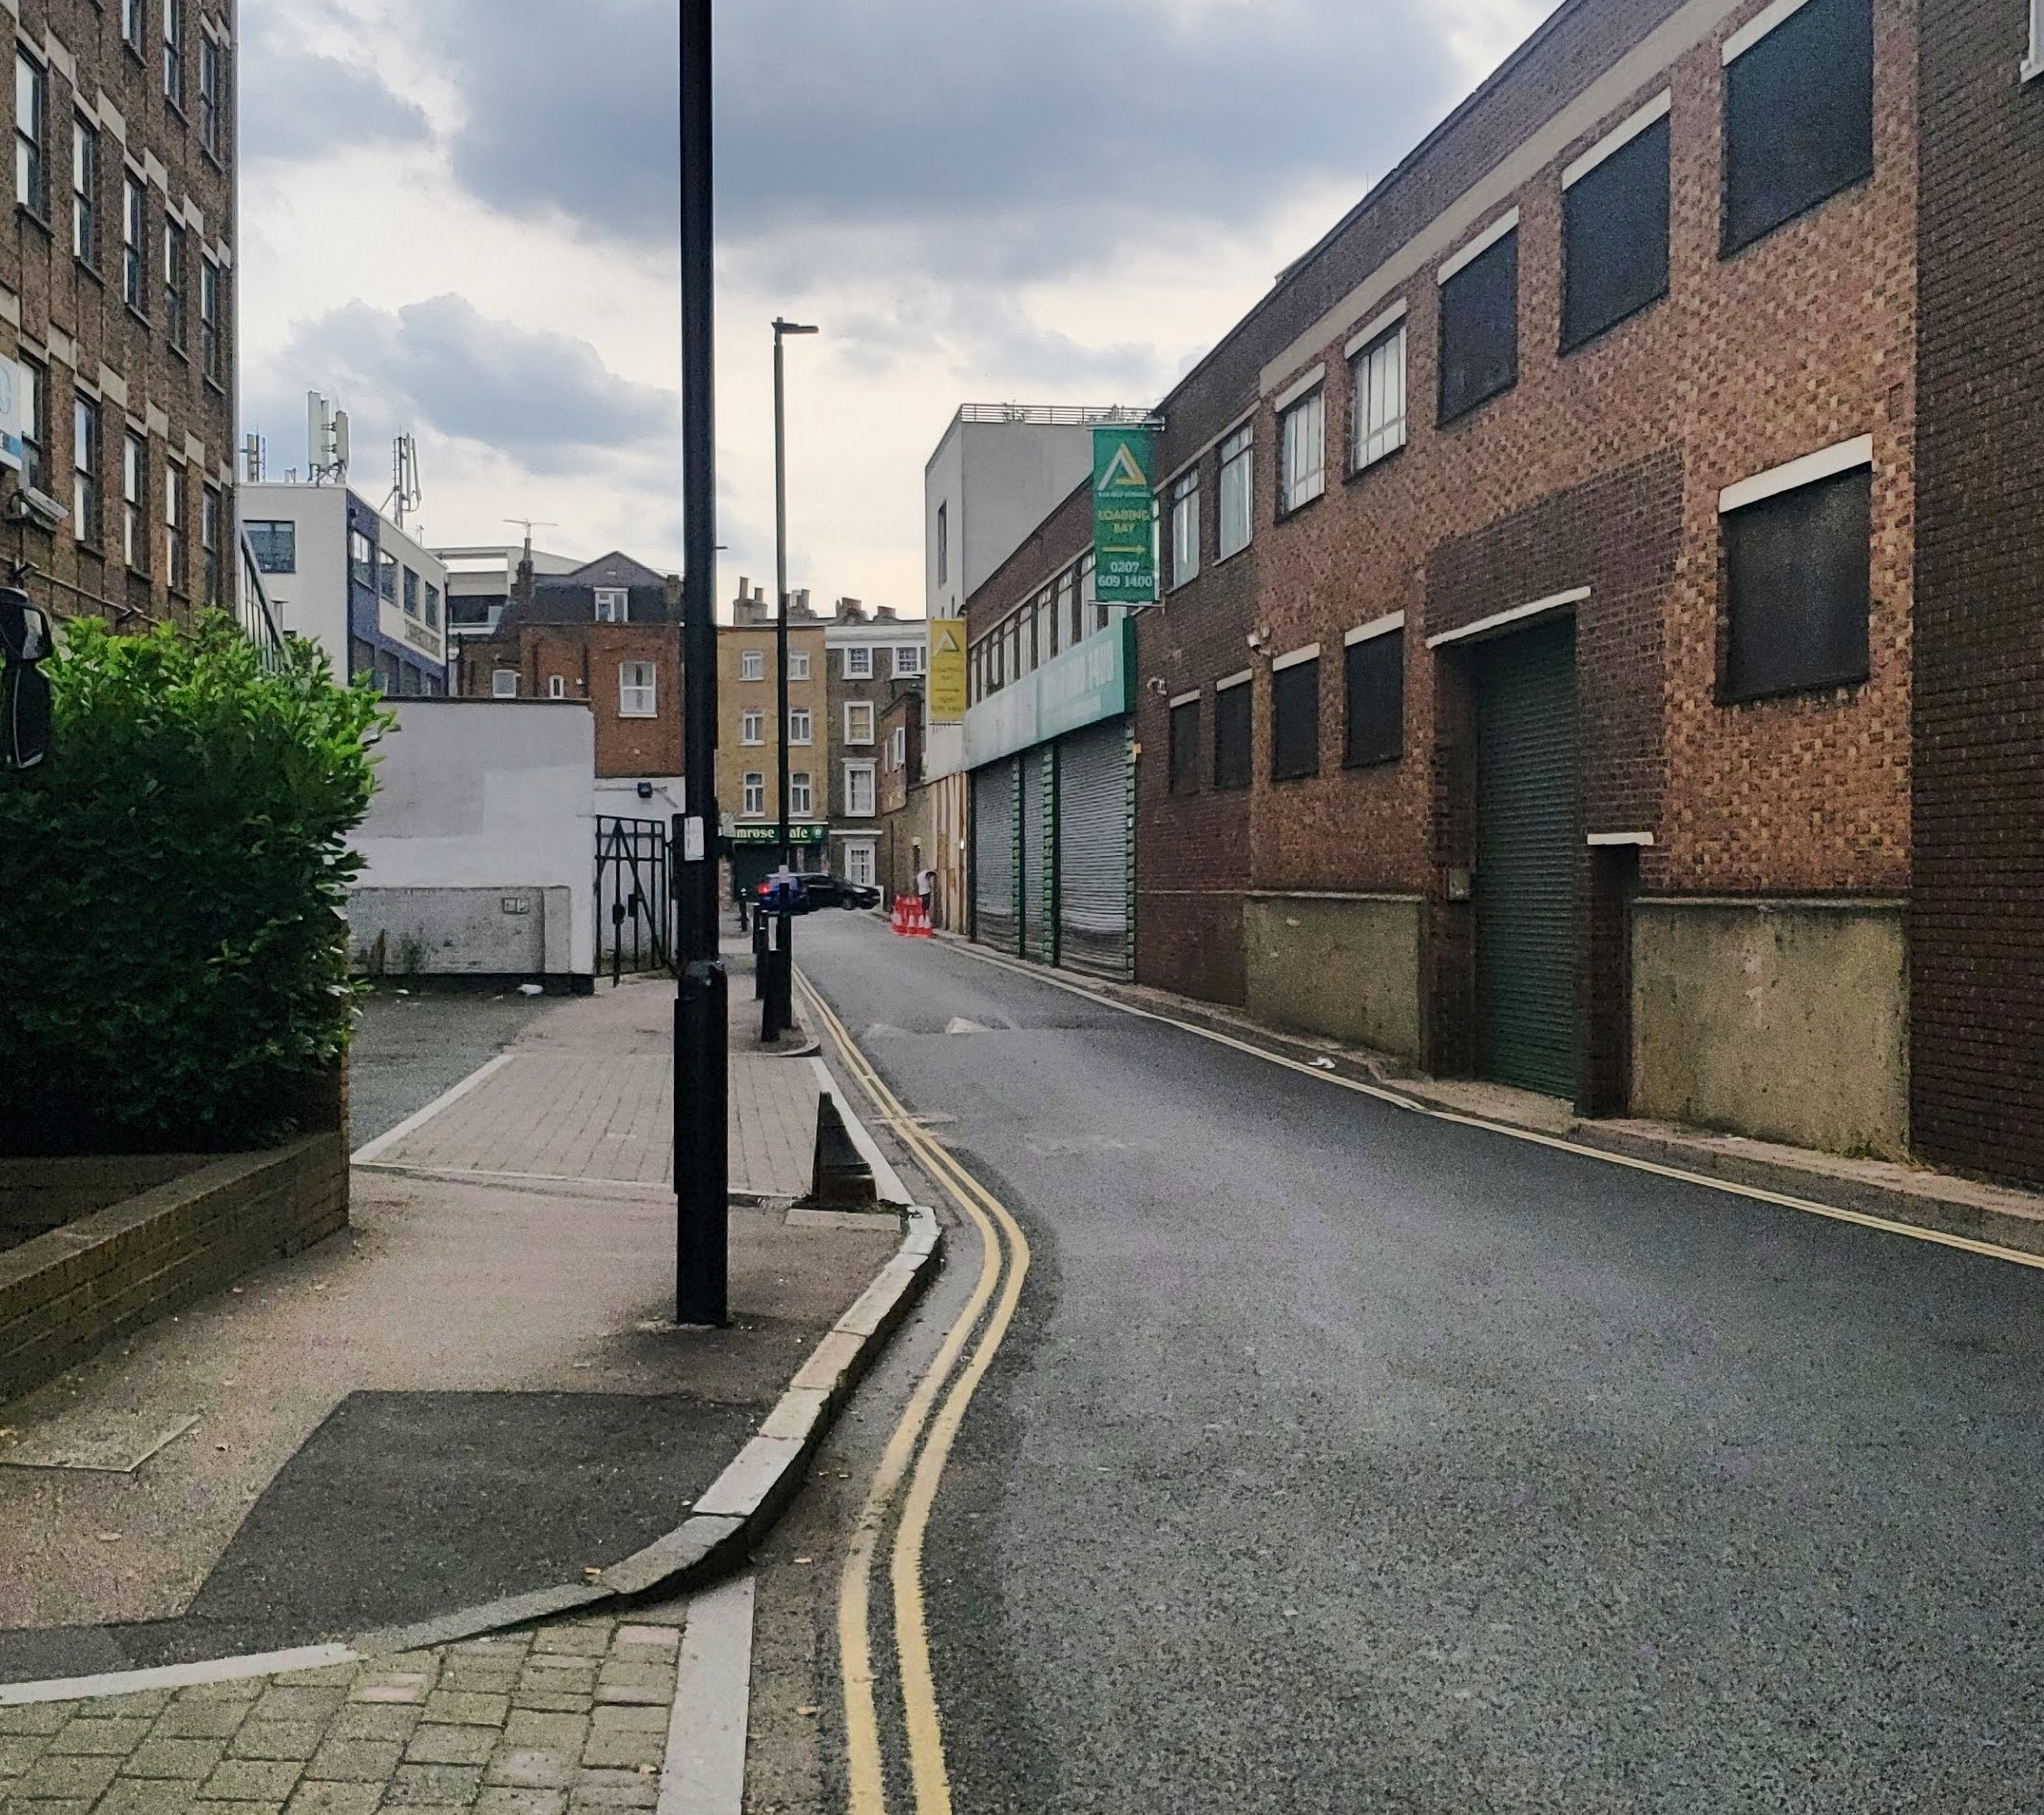
\includegraphics[width=0.6\textwidth]{brandon_rd_cropped}
\caption{image of quietway}
\end{figure}

\begin{figure}
\centering
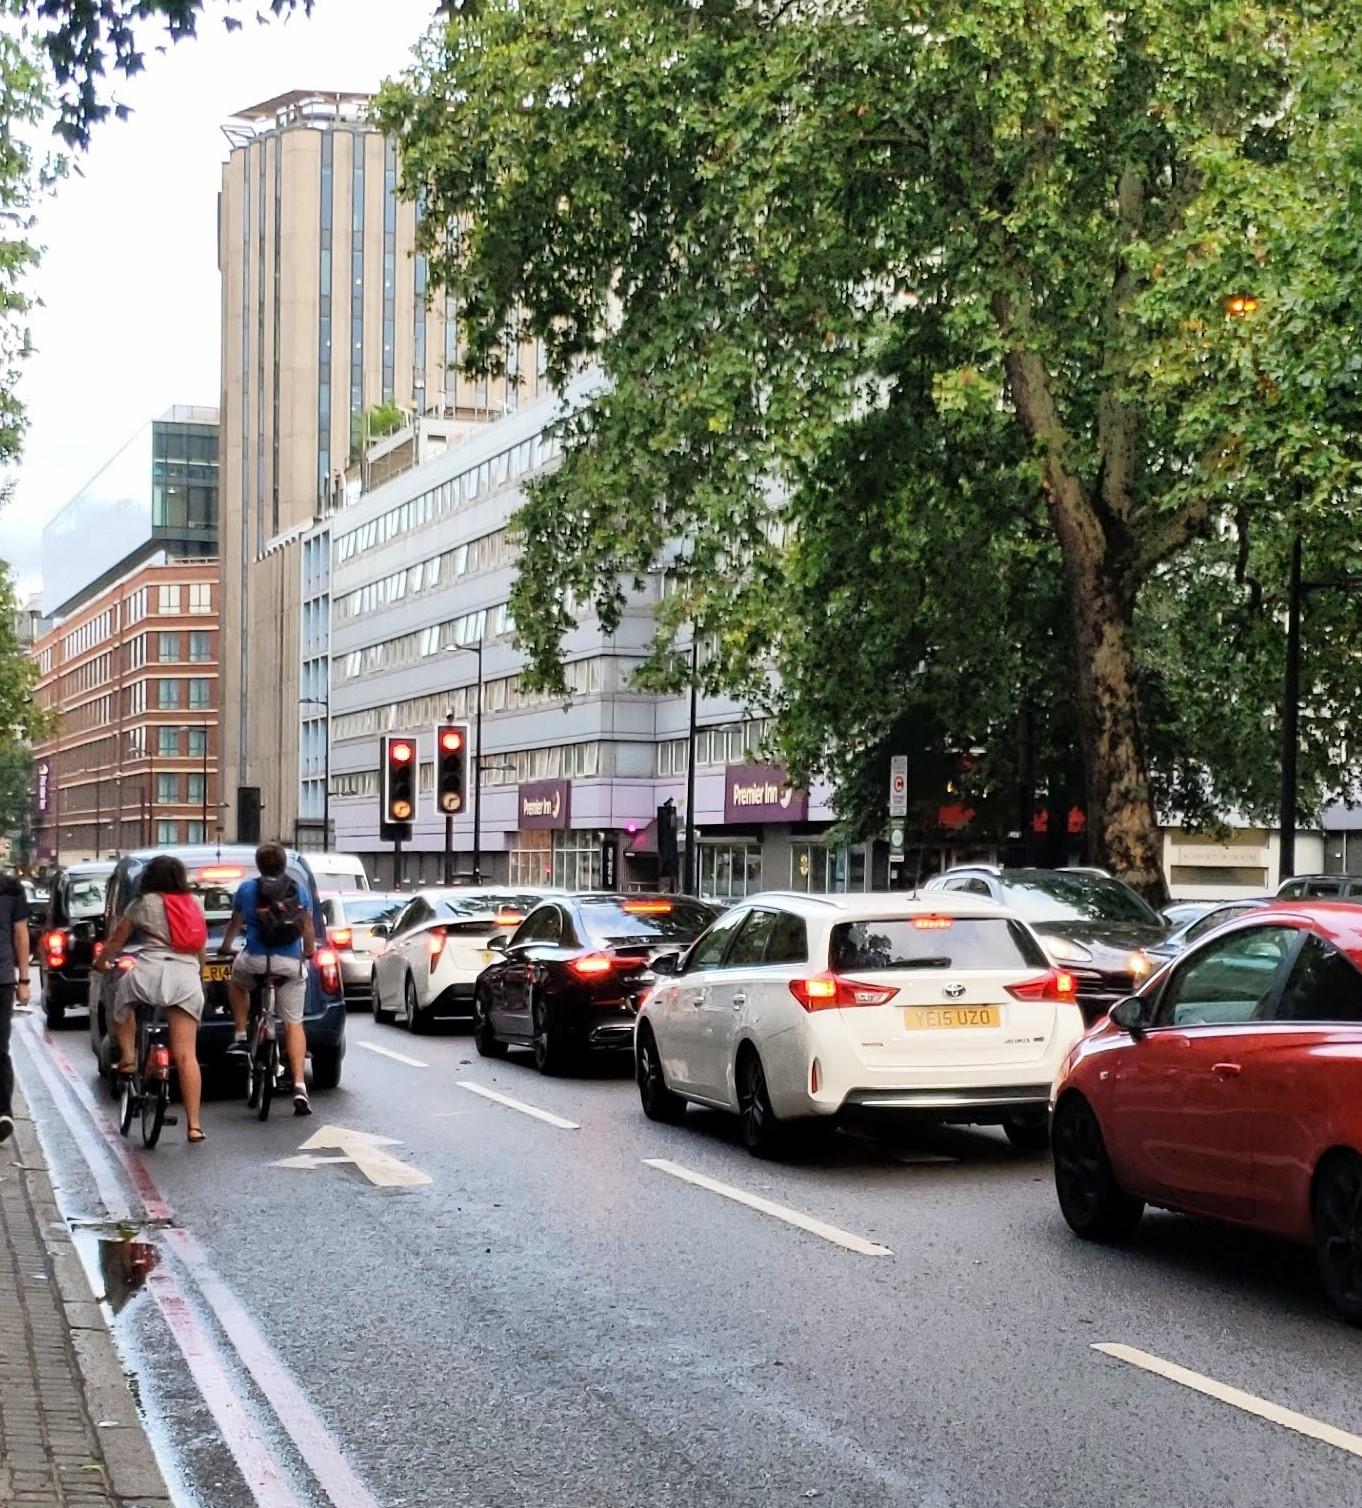
\includegraphics[width=0.6\textwidth]{euston_rd_cropped}
\caption{An image of Euston Road}
\label{fig:euston}
\end{figure}

\subsection{Transport for London Cycling Infrastructure Database}

\cite{tflcid}

This data was in the process of being publishing during the period of research for this work. While it was not available at the time of publication, it is notable because it promises to raise the quality and volume of OSM data for London substantially. It includes 2,000km of cycle lanes as well as hundreds of thousands of parking spaces, cycling related signs and other relevant features. \cite{osmtflcidwiki}. 

Section XXXX from the Lit Review addressed to possibility for bulk data uploads to dramatically enhance OSM data quality and this may be one example. The data was professionally surveyed. 

\subsection{QUANT}

The QUANT dataset of public transport travel times was .

CITE

The of 22 million pairs, 5.8 million pairs had no public transport link. To clean this data, the set is cut down to match the scope of the the investigation. Where there is no link between an origin destination pair, a link is constructed by combining the walking time from the origin to the node of highest degree in another LSOA where public transport is available to the destination LSOA. 

The walking speed used will be taken from google and the distance is the straight-line distance between two points. This is less accurate than actually finding the walking route between the two points but this level of detail was not computationally feasible. 

The QUANT data provides a point of comparison for cycling travel times to be calculated. 

\subsection{2011 Census Journey to work data}

The 2011 census asked each household where they lived, where they worked and how they traveled to work the preceding week (\cite{jtw}). Thus data for origin and destination by mode of transport was available. This data will be used to help define the optimal scope as well as to compute a ``connectivity ratio'' like that of \cite{furth2012low} for a network. 

This data is shared through the Nomis Labor Force website as multi-sheet excel pivot tables. Making the data usable required, stripping the meta data headings from each sheet, importing the book to pandas dataframe by sheet, melting from a pivot table to long data with origin, destination, and count columns, adding the sheet name that identified the mode of travel as a column, appending each individual sheet together into a single dataframe, and pushing the dataframe to the sql database. 

\subsection{LSOA boundaries and data}
	
LSOA boundaries were obtained from  \cite{lsoageoms}. The LSOA boundareis were determined as a part of the 2011 census containing approximately 5000 people each. These are used, first to specify a boundary for the scope of the study and then to specify origin and destination nodes on the network. The node closest to the centroid of each LSOA is selected as the origin and destination or that LSOA. Where LSOA's were comprised of multiple polygons, the centroid of the largest polygon was used. These polygons were used for the production of maps seen in the Analysis section XXXXX. 

On maps created using these boundaries the copyright must be stated. This is
%"Contains National Statistics data © Crown copyright and database right [2015]" and "Contains Ordnance Survey data © Crown copyright and database right [2015]"
	
\subsection{Road KSI data}

Data on those killed or seriously injured on London streets is available through CITE. This was used to assist in determining the scope of the investigation. While it was hoped that the data could be used to build an estimate of danger to cyclists on London's streets several obstacles prevented this. The first is the change in infrastructure over time and lack of data about the exact infrastructure present at the time and location of each incident. Second was the lack of high resolution data about cyclist volumes. An area that has a particularly high KSI rate may be especially dangerous or may be relatively safe after adjusted for cyclist miles traveled, an unknown. London has begun collecting some data on cyclist volumes although this remains fairly sparse. \cite{cyclistksi}
	
\subsection{Data import, storage, cleaning, and joining}

data import was done in python using the csv, pandas, geopandas, json, and osmnx packages. 
Data from OSM was converted from json to a dataframe, tags simplified, edges truncated, geometry simplified. 
Geometry was converted to well known text and multi-lines were broken into several single line geometries for compatibility with the postgis databse. 

Once the data was cleaned, it was passed to a postgres database with the postgis extension using the sqlalchemy package. Postgis was used for calculating distances, associating nodes with centroids. 

remove multipolygon lsoa interior rings in favor of polygon lsoa shapes

QGIS was used to melt polygons into outer boundary and for the construction of visualizations

cite postgres
\cite{postgres}
cite postgis
\cite{postgis}
cited dbeaver
\cite{dbeaver}
cite python
\cite{python}
cite pandas
\cite{pandas}
cite json

cite sqlachemy
\cite{bayer2010sqlalchemy}
cite qgis
\cite{qgis}